\section{\RU{Вложенные структуры}\EN{Nested structures}}

\RU{Теперь, как насчет ситуаций, когда одна структура определена внутри другой структуры?}
\EN{Now what about situations when one structure is defined inside of another?}

\lstinputlisting{patterns/15_structs/5_nested/nested.c}

\dots \RU{в этом случае, оба поля \TT{inner\_struct} просто будут располагаться между полями a,b и d,e в 
\TT{outer\_struct}.}
\EN{in this case, both \TT{inner\_struct} fields are to be placed between the a,b and d,e fields of
the \TT{outer\_struct}.}

\RU{Компилируем}\EN{Let's compile} (MSVC 2010):

\lstinputlisting[caption=\Optimizing MSVC 2010 /Ob0]{patterns/15_structs/5_nested/nested_msvc.asm}

\RU{Очень любопытный момент в том, что глядя на этот код на ассемблере, мы даже не видим, 
что была использована какая-то еще другая структура внутри этой!
Так что, пожалуй, можно сказать, что все вложенные структуры в итоге разворачиваются в одну, \IT{линейную} 
или \IT{одномерную} структуру.}
\EN{One curious thing here is that by looking onto this assembly code, we do not even see that
another structure was used inside of it!
Thus, we would say, nested structures are unfolded into \IT{linear} or \IT{one-dimensional} structure.}

\RU{Конечно, если заменить объявление \TT{struct inner\_struct c;} на \TT{struct inner\_struct *c;} 
(объявляя таким образом указатель), ситуация будет совсем иная.}
\EN{Of course, if we replace the \TT{struct inner\_struct c;} declaration with \TT{struct inner\_struct *c;} 
(thus making a pointer here) the situation will be quite different.}
% FIXME1: нарисовать вложенную структуру и развернутую

\ifdefined\IncludeOlly
\clearpage
\subsection{\olly}
\index{\olly}

\RU{Загружаем пример в}\EN{Let's load the example into} \olly \RU{и смотрим на}\EN{and take a look at} 
\TT{outer\_struct} \RU{в памяти}\EN{in memory}:

\begin{figure}[H]
\centering
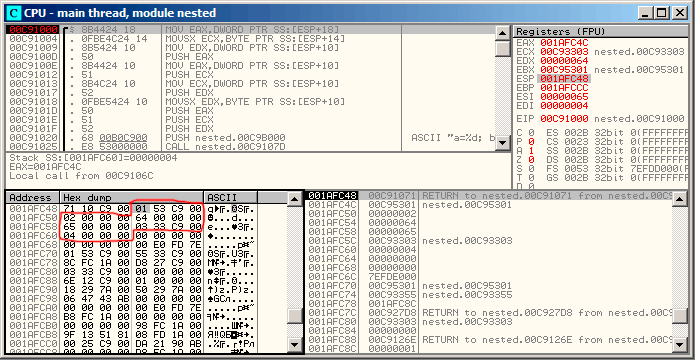
\includegraphics[scale=\FigScale]{patterns/15_structs/5_nested/olly.png}
\caption{\olly: \RU{Перед исполнением \printf}\EN{Before \printf execution}}
\label{fig:nested_olly}
\end{figure}

\RU{Вот как расположены значения в памяти}\EN{That's how the values are located in memory}:
\begin{itemize}
\item \IT{(outer\_struct.a)} \RU{(байт) 1 + 3 байта случайного мусора}\EN{(byte) 1 + 3 bytes of random garbage};
\item \IT{(outer\_struct.b)} (\RU{32-битное слово}\EN{32-bit word}) 2;
\item \IT{(inner\_struct.a)} (\RU{32-битное слово}\EN{32-bit word}) 0x64 (100);
\item \IT{(inner\_struct.b)} (\RU{32-битное слово}\EN{32-bit word}) 0x65 (101);
\item \IT{(outer\_struct.d)} \RU{(байт) 3 + 3 байта случайного мусора}\EN{(byte) 3 + 3 bytes of random garbage};
\item \IT{(outer\_struct.e)} (\RU{32-битное слово}\EN{32-bit word}) 4.
\end{itemize}

\fi

